\documentclass[9pt]{article}

\usepackage{amssymb}
\usepackage{amsmath}
\usepackage{amsfonts}
\usepackage{comment}
\usepackage{fancyhdr}
\usepackage{mathrsfs}
\usepackage{graphicx}

\voffset = -50pt
%\textheight = 700pt
\addtolength{\textwidth}{60pt}
\addtolength{\evensidemargin}{-30pt}
\addtolength{\oddsidemargin}{-30pt}
%\setlength{\headheight}{44pt}

\pagestyle{fancy}
\fancyhf{} % clear all fields
\fancyhead[R]{%
  \scshape
  \begin{tabular}[t]{@{}r@{}}
  CECS 285, Spring 2015\\Section 1 (4344)\\
  Lab \#6, Due: 2015, March 11
  \end{tabular}}
\fancyhead[L]{%
  \scshape
  \begin{tabular}[t]{@{}r@{}}
  JOSEPH OKONOBOH, 013755064\\Computer Science\\Cal State Long Beach
  \end{tabular}}
\fancyfoot[C]{\thepage}

\begin{document}
\begin{enumerate}
%%%%%%%%%%%%%%%%%%%%%%%%%%%%%%%%%%%%%Prob1%%%%%%%%%%%%%%%%%%%%%%%%%%%%%%%%%%%%%%
   \item \begin{tabular}{@{}|c|c|c|c|@{}}
            \hline \textbf{Switch value in binary} & \textbf{PWM Duty Cycle} &
                   \textbf{Numerator} & \textbf{Denominator} \\
            \hline \verb|000| & \verb|11%| & \verb|Y1=1| & \verb|X=9| \\
            \hline \verb|001| & \verb|22%| & \verb|Y1=2| & \verb|X=9| \\
            \hline \verb|010| & \verb|33%| & \verb|Y1=3| & \verb|X=9| \\
            \hline \verb|011| & \verb|44%| & \verb|Y1=4| & \verb|X=9| \\
            \hline \verb|100| & \verb|55%| & \verb|Y1=5| & \verb|X=9| \\
            \hline \verb|101| & \verb|66%| & \verb|Y1=6| & \verb|X=9| \\
            \hline \verb|110| & \verb|77%| & \verb|Y1=7| & \verb|X=9| \\ 
            \hline \verb|111| & \verb|88%| & \verb|Y1=8| & \verb|X=9| \\ \hline
         \end{tabular}
   \item To get the required delay time, let us consider the snippet of code
         below for yet to be determined positive integers $x$ and $y$.
         \begin{verbatim}
DELAY:
                  MOV R0, #x
         LOOP0:   MOV R1, #y
         LOOP1:   DJNZ R1, LOOP1
                  DJNZ R0, LOOP0
         \end{verbatim}
         The number of machine cycles for this code is
         $$2 + [2 + 4 \cdot y + 4] \cdot x = 4xy + 6x + 2.$$
         Since we our machine is a DS89C450 and since we want to generate a
         $\displaystyle\frac{1}{5400} s$ delay time, we must have that
         $$(4xy + 6x + 2) \cdot 90.42 ns = \frac{1}{5400}.$$
         So choose $x = 11$ and solve to get $y \approx 45$.
   \item \begin{verbatim}
   
   
   
         ;;;;;;;;;;;;;;;;;;;;;;;;;;;;;;;;;;;;;;;;;;;;;;;;;;;;;;;;;;;;;;;;;;;;;;;
         ;;;;;;;;;;;;;;;;;;;;;;;;;PULSE-MODULATION CODE;;;;;;;;;;;;;;;;;;;;;;;;;
         ;;;;;;;;;;;;;;;;;;;;;;;;;;;;;;;;;;;;;;;;;;;;;;;;;;;;;;;;;;;;;;;;;;;;;;;
   
         MOV      P0, #0         ;Set Port 0 as output
         MOV      P1, #07H       ;Use low 3-bit of P1 for modulation

MAIN_LOOP:
         MOV      R2, P1         ;Read data from switch into R2
         INC      R2             ;Add 1 to get index of switch
         MOV      P0, #0FFH      ;Turn on LEDs

DELAY_ON:
         ACALL    DELAY          ;Keep LEDs on for R2 * Delay time
         DJNZ     R2, DELAY_ON
				
         MOV      R2, P1         ;Read data from switch into R2
			
         MOV      A, #8					
         SUBB     A, R2          ;Off Time = (8 - R2) * Delay time
         MOV      R2, A	
         
         MOV      P0, #0         ;Turn off LEDs
	
DELAY_OFF:
         ACALL    DELAY          ;Keep LEDs on for R2 * Delay time
         DJNZ     R2, DELAY_OFF	
			
         SJMP MAIN_LOOP						

DELAY:
                  MOV R0, #11    ;Delay time for DS89C450 at 600 Hz
         LOOP0:
                  MOV R1, #45    
         LOOP1:
                  DJNZ R1, LOOP1 
                  DJNZ R0, LOOP0
         RET
END
         \end{verbatim}
   \item \textbf{Flow Chart} \text{ } \\
                  \begin{center}
                     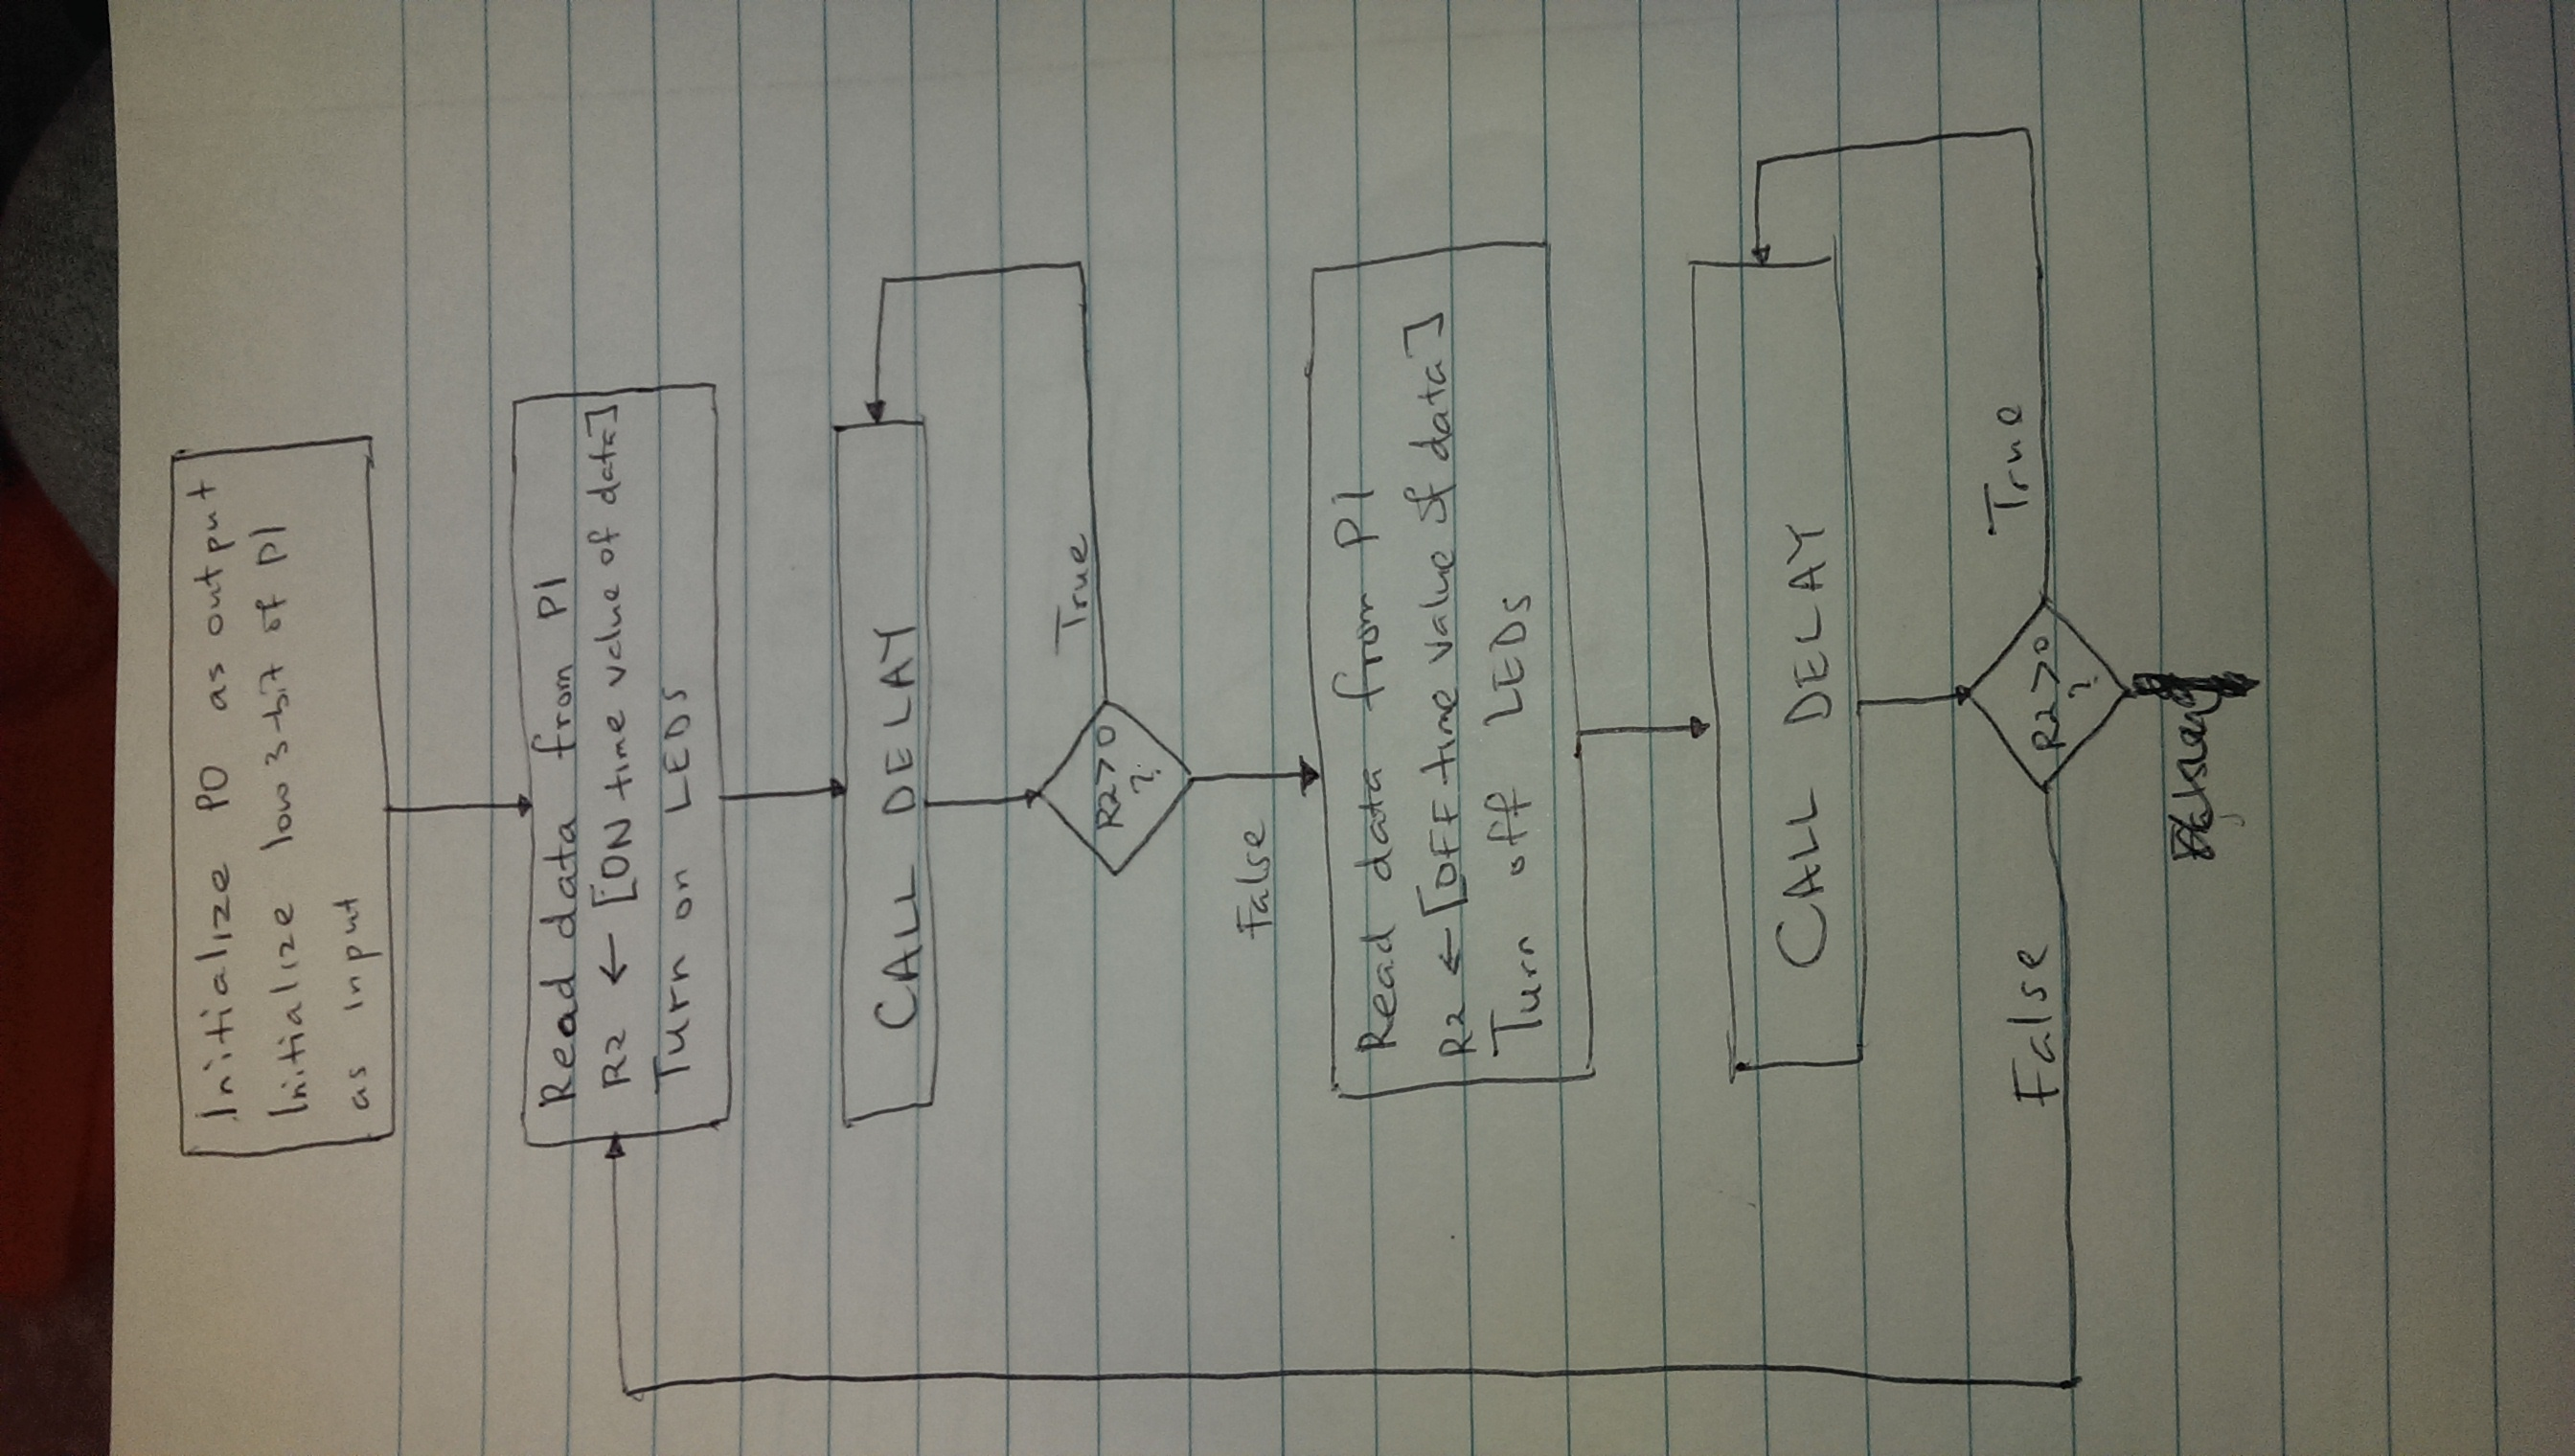
\includegraphics[angle=-90,width=\textwidth]{flowchart.jpg}
                  \end{center}
\end{enumerate}
\end{document}
